\let\negmedspace\undefined
\let\negthickspace\undefined
\documentclass[journal]{IEEEtran}
\usepackage[a5paper, margin=10mm, onecolumn]{geometry}
%\usepackage{lmodern} % Ensure lmodern is loaded for pdflatex
\usepackage{tfrupee} % Include tfrupee package

\setlength{\headheight}{1cm} % Set the height of the header box
\setlength{\headsep}{0mm}     % Set the distance between the header box and the top of the text

\usepackage{gvv-book}
\usepackage{gvv}
\usepackage{cite}
\usepackage{amsmath,amssymb,amsfonts,amsthm}
\usepackage{algorithmic}
\usepackage{graphicx}
\usepackage{textcomp}
\usepackage{xcolor}
\usepackage{txfonts}
\usepackage{listings}
\usepackage{enumitem}
\usepackage{mathtools}
\usepackage{gensymb}
\usepackage{comment}
\usepackage[breaklinks=true]{hyperref}
\usepackage{tkz-euclide} 
\usepackage{listings}
% \usepackage{gvv}                                        
\def\inputGnumericTable{}                                 
\usepackage[latin1]{inputenc}                                
\usepackage{color}                                            
\usepackage{array}                                            
\usepackage{longtable}                                       
\usepackage{calc}                                             
\usepackage{multirow}                                         
\usepackage{hhline}                                           
\usepackage{ifthen}                                           
\usepackage{lscape}
\usepackage{circuitikz}
\tikzstyle{block} = [rectangle, draw, fill=blue!20, 
    text width=4em, text centered, rounded corners, minimum height=3em]
\tikzstyle{sum} = [draw, fill=blue!10, circle, minimum size=1cm, node distance=1.5cm]
\tikzstyle{input} = [coordinate]
\tikzstyle{output} = [coordinate]


\begin{document}

\bibliographystyle{IEEEtran}
\vspace{3cm}

\title{9-9.6-17}
\author{EE24BTECH11064 - Harshil Rathan}
 \maketitle
% \newpage
% \bigskip
{\let\newpage\relax\maketitle}

\renewcommand{\thefigure}{\theenumi}
\renewcommand{\thetable}{\theenumi}
\setlength{\intextsep}{10pt} % Space between text and floats


\numberwithin{equation}{enumi}
\numberwithin{figure}{enumi}
\renewcommand{\thetable}{\theenumi}

\textbf{Question}:\\
Find the equation of a curve passing through the point (0, 2) given that the sum of the coordinates of any point on the curve exceeds the magnitude of the slope of the tangent to the curve at that point by 5. \\ 
\solution \\
Let us solve the given equation theoretically and then verify the solution computationally \\
According to the question, \\
Sum of the coordinates of any point say $\brak{x,y}$ on the curve = Magnitude of the slope of the tangent to the curve + 5 
\begin{align}
    x+y = \frac{dy}{dx} + 5 
\end{align}
\begin{align}
    \frac{dy}{dx} - y= x-5
    \label{0.2}
\end{align}
Comparing \ref{0.2} with $\frac{dy}{dx} + Py = Q$
\begin{align}
    P=-1 \text{ and } Q=x-5
\end{align}
I.F is \ref{0.4}
\begin{align}
    e^{\int P dx} = e^ {-x}
    \label{0.4}
\end{align}
Solution is \ref{0.6}
\begin{align}
    y\text{ }(I.F) = \int Q\text{ }(I.F)\text{ }dx + c 
\end{align}
\begin{align}
    y \cdot e^{-x} = \int \brak{x-5} e^{-x} \text{ }dx +c 
    \label{0.6}
\end{align}
Apply product rule :
\begin{align}
    \int A\cdot B \text{ }dx = A \int B \text{ }dx - \int \frac{d}{dx}(A)\brak{\int B \text{ }dx}dx
\end{align}
\begin{align}
     y e^{-x} = - (x-5)e^{-x} + \int e^{-x}  dx + c
 \end{align}
\begin{align}
     y e^{-x} = - (x-5)e^{-x} + \frac{e^{-x}}{-1} + c 
\end{align}
\begin{align}
     \frac{y}{(e^x)}= - \frac{(x-5)}{(e^{x})} - \frac{1}{e^x} + c
\end{align}
On Simplifying 
\begin{align}
     y = - (x-5) - 1 +c e^x
\end{align}
\begin{align}
    x+y = 4 + c e^x
    \label{0.12}
\end{align}
To find c, put x=0 and y=2 in \ref{0.12}
\begin{align}
    c = -2  
\end{align}
The curve is 
\begin{align}
   x+y = 4 -2e^x
\end{align}


\textbf{Solution using Laplace transform method}\\
\begin{align}
    \frac{dy}{dx} = x+y-5
\end{align}
Applying the Laplace transform to both sides:

\begin{align}
    \mathcal{L}\left\{\frac{dy}{dx}\right\} = \mathcal{L}\left\{x + (y - 5)\right\}
\end{align}
\begin{align}
    sY(s) - y(0) = \frac{1}{s^2} + Y(s) - \frac{5}{s}
\end{align}
\begin{align}
    Y(s) = \frac{\frac{1}{s^2} - \frac{5}{s} + y(0)}{s - 1}
\end{align}
\begin{align}
    Y(s) = \frac{1}{s^2 (s - 1)} - \frac{1}{s (s - 1)} \cdot 5 + \frac{y(0)}{s - 1}
\end{align}
Inverse Laplace Transform of Each Term
\begin{align}
    \frac{1}{s^2 (s - 1)} = \frac{A}{s} + \frac{B}{s^2} + \frac{C}{s - 1}
\end{align}
\begin{align}
    1 = A\text{ } s\text{ } (s - 1) + B \text{ }(s - 1) + C \text{ }s^2
\end{align}
we get
\begin{align}
    \frac{1}{s^2 (s - 1)} = -\frac{1}{s} -\frac{1}{s^2} + \frac{1}{s - 1}
\end{align}
Taking the inverse Laplace transform
\begin{align}
    \mathcal{L}^{-1}\left\{ \frac{1}{s} - \frac{1}{s - 1} \right\} = -1 - x + e^x
\end{align}
Inverse Laplace of \( \frac{5}{s (s - 1)} \)
\begin{align}
    \frac{5}{s (s - 1)} = \frac{A}{s} + \frac{B}{s - 1}
\end{align}
\begin{align}
    5 = A (s - 1) + B s
\end{align}
Solving gives \( A = 5 \) and \( B = -5 \)
\begin{align}
    \frac{5}{s (s - 1)} = \frac{5}{s} - \frac{5}{s - 1}
\end{align}
Taking the inverse Laplace transform
\begin{align}
    \mathcal{L}^{-1}\left\{ \frac{5}{s} - \frac{5}{s - 1} \right\} = 5 - 5 e^x
\end{align}
Inverse Laplace of \( \frac{y(0)}{s - 1} \)
\begin{align}
    \mathcal{L}^{-1}\left\{ \frac{y(0)}{s - 1} \right\} = y(0) e^x
\end{align}
combining the results from all parts, we have the solution for $y(x)$
The general solution too this differential equation is 
\begin{align}
    y(x) = 4 - x + (y(0) - 4) e^x \\
    y(x) = 4 - x + c  e^x
    \label{0.30}
\end{align}
To find c, put x=0 and y=2 in \ref{0.30}
\begin{align}
    c = -2  
\end{align}
The curve is 
\begin{align}
   x+y = 4 -2e^x
\end{align}
Now lets verify the solution computationally from the definition of $\frac{dy}{dx}$
\begin{align}
    y_{n+1}= y_{n} + \frac{dy}{dx} \cdot h
    \label{0.21}
\end{align}
From the differential equation given,
\begin{align}
    \frac{dy}{dx} = x+y-5
    \label{0.22}
\end{align}
Substituting \ref{0.22} in \ref{0.21}
\begin{align}
    y_{n+1} = y_n + \brak{x_n + y_n -5} \cdot h 
\end{align}
From the figure it is clearly verified that the theoretical solution matches with the computational solution\\
\begin{figure}
    \centering
    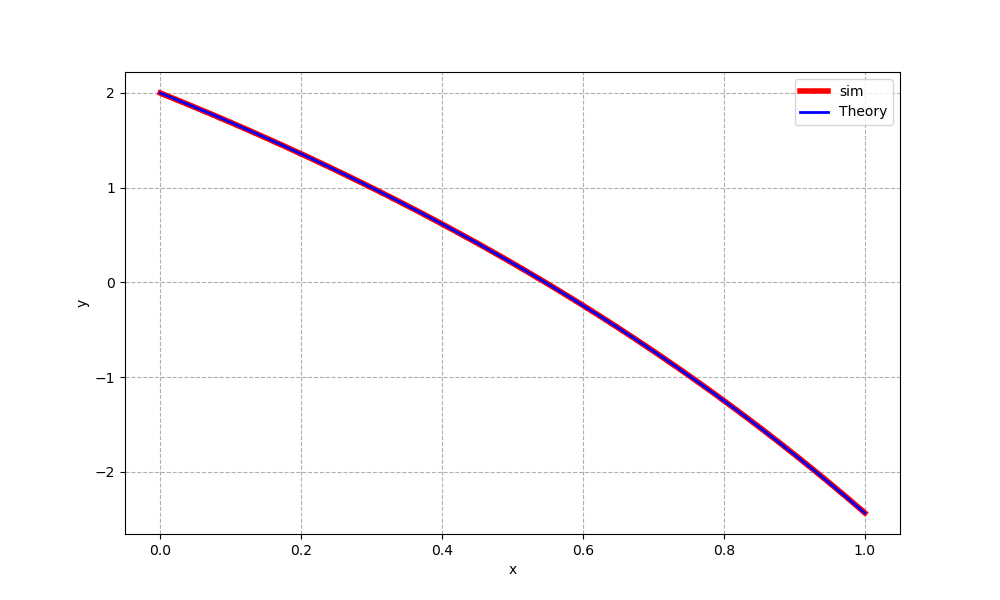
\includegraphics[width=\columnwidth]{figs/Figure_1.png}
\end{figure}
\end{document}



